\newcommand{\DrawConfiguration}[6]{
    \begin{scope}[xshift=#1, yshift=#2]
        \draw[step=2,black,thin] (-1,-1) grid (1,1);
        \node[#3] at ( 0.5,  0.0) {};
        \node[#4] at ( 0.0,  0.5) {};
        \node[#5] at (-0.5,  0.0) {};
        \node[#6] at ( 0.0, -0.5) {};
    \end{scope}
}
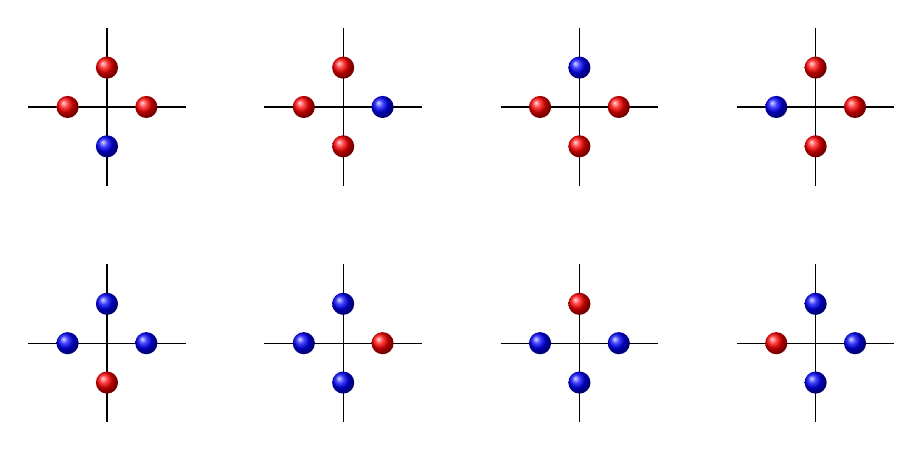
\begin{tikzpicture}[
  ball/.style={shade, shading=ball, circle, minimum size=8pt, inner sep=0pt},
  zero/.style={ball, ball color=red},
  one/.style={ball, ball color=blue}
  ]
  \DrawConfiguration{0cm}{3cm}{zero}{zero}{zero}{one}
  \DrawConfiguration{3cm}{3cm}{one}{zero}{zero}{zero}
  \DrawConfiguration{6cm}{3cm}{zero}{one}{zero}{zero}
  \DrawConfiguration{9cm}{3cm}{zero}{zero}{one}{zero}
  \DrawConfiguration{0cm}{0cm}{one}{one}{one}{zero}
  \DrawConfiguration{3cm}{0cm}{zero}{one}{one}{one}
  \DrawConfiguration{6cm}{0cm}{one}{zero}{one}{one}
  \DrawConfiguration{9cm}{0cm}{one}{one}{zero}{one}
\end{tikzpicture}
